

\tikzset{every picture/.style={line width=0.3pt}} %set default line width to 0.75pt        

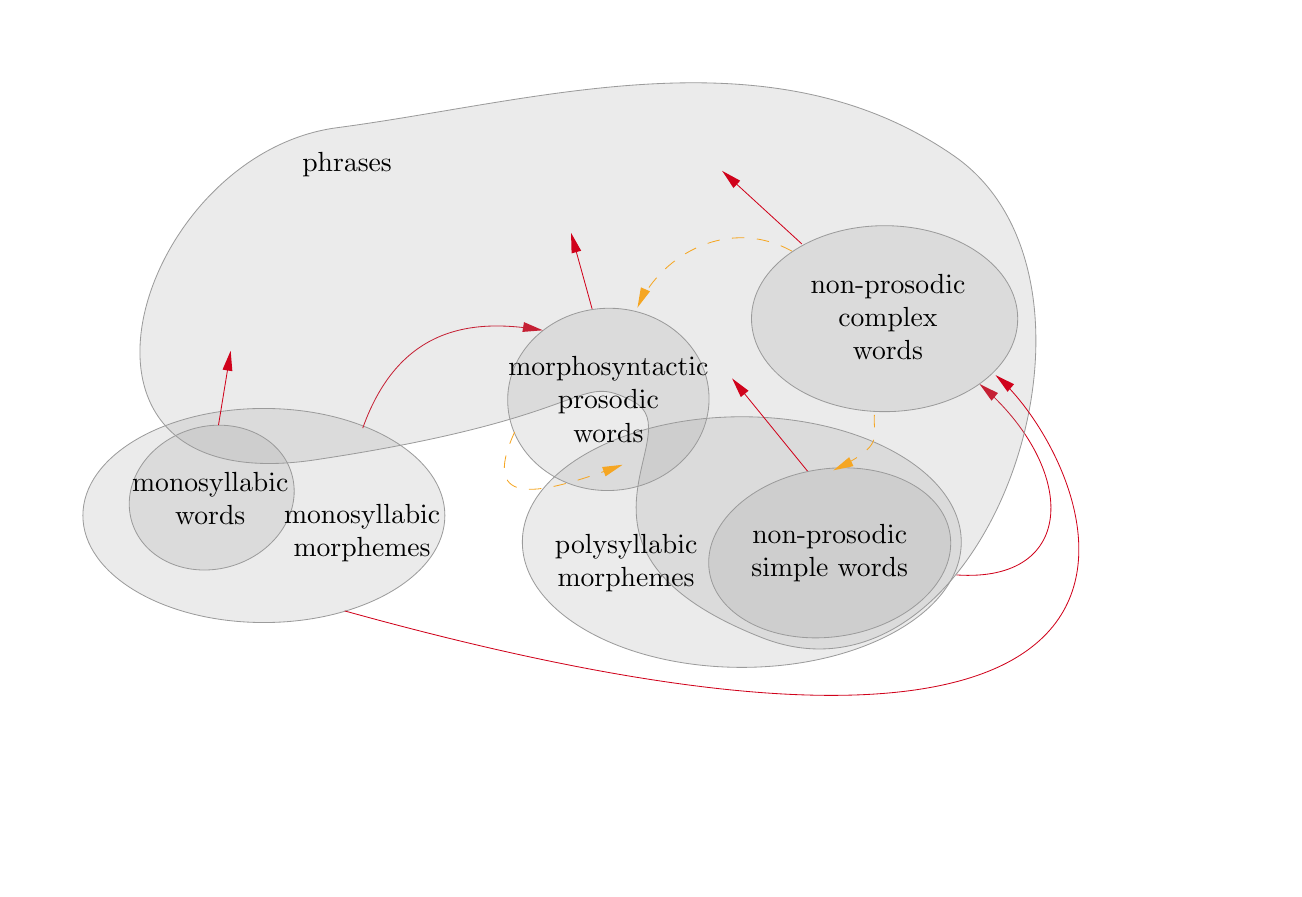
\begin{tikzpicture}[x=0.75pt,y=0.75pt,yscale=-0.8,xscale=0.8]
%uncomment if require: \path (0,665); %set diagram left start at 0, and has height of 665

%Shape: Ellipse [id:dp16595835288380223] 
\draw  [color={rgb, 255:red, 155; green, 155; blue, 155 }  ,draw opacity=1 ][fill={rgb, 255:red, 155; green, 155; blue, 155 }  ,fill opacity=0.2 ] (66.33,375.46) .. controls (66.33,339.86) and (115.13,311) .. (175.33,311) .. controls (235.53,311) and (284.33,339.86) .. (284.33,375.46) .. controls (284.33,411.07) and (235.53,439.93) .. (175.33,439.93) .. controls (115.13,439.93) and (66.33,411.07) .. (66.33,375.46) -- cycle ;
%Shape: Ellipse [id:dp6777440286998517] 
\draw  [color={rgb, 255:red, 155; green, 155; blue, 155 }  ,draw opacity=1 ][fill={rgb, 255:red, 155; green, 155; blue, 155 }  ,fill opacity=0.2 ] (331,391.46) .. controls (331,349.79) and (390.17,316) .. (463.17,316) .. controls (536.16,316) and (595.33,349.79) .. (595.33,391.46) .. controls (595.33,433.14) and (536.16,466.93) .. (463.17,466.93) .. controls (390.17,466.93) and (331,433.14) .. (331,391.46) -- cycle ;
%Shape: Ellipse [id:dp24014776883482214] 
\draw  [color={rgb, 255:red, 155; green, 155; blue, 155 }  ,draw opacity=1 ][fill={rgb, 255:red, 155; green, 155; blue, 155 }  ,fill opacity=0.2 ] (156.54,405.71) .. controls (130.02,413.87) and (102.86,402.13) .. (95.89,379.47) .. controls (88.91,356.82) and (104.76,331.83) .. (131.29,323.67) .. controls (157.81,315.5) and (184.97,327.25) .. (191.94,349.9) .. controls (198.92,372.56) and (183.07,397.54) .. (156.54,405.71) -- cycle ;
%Shape: Ellipse [id:dp7785114628637544] 
\draw  [color={rgb, 255:red, 155; green, 155; blue, 155 }  ,draw opacity=1 ][fill={rgb, 255:red, 155; green, 155; blue, 155 }  ,fill opacity=0.2 ] (384.9,360.39) .. controls (351.42,361.67) and (323.35,338.15) .. (322.19,307.86) .. controls (321.03,277.57) and (347.23,251.98) .. (380.7,250.7) .. controls (414.18,249.42) and (442.25,272.94) .. (443.41,303.23) .. controls (444.57,333.52) and (418.37,359.11) .. (384.9,360.39) -- cycle ;
%Shape: Ellipse [id:dp22063005189030394] 
\draw  [color={rgb, 255:red, 155; green, 155; blue, 155 }  ,draw opacity=1 ][fill={rgb, 255:red, 155; green, 155; blue, 155 }  ,fill opacity=0.2 ] (443.63,409.27) .. controls (439.32,381.69) and (468.27,354.26) .. (508.29,348.01) .. controls (548.31,341.76) and (584.25,359.05) .. (588.56,386.63) .. controls (592.87,414.21) and (563.92,441.64) .. (523.9,447.89) .. controls (483.88,454.14) and (447.94,436.85) .. (443.63,409.27) -- cycle ;
%Curve Lines [id:da7046092630449821] 
\draw [color={rgb, 255:red, 208; green, 2; blue, 27 }  ,draw opacity=1 ]   (234.86,322.86) .. controls (257.98,257.92) and (305.87,257.91) .. (341.7,263.66) ;
\draw [shift={(343.33,263.93)}, rotate = 189.46] [fill={rgb, 255:red, 208; green, 2; blue, 27 }  ,fill opacity=1 ][line width=0.08]  [draw opacity=0] (12,-3) -- (0,0) -- (12,3) -- cycle    ;
%Curve Lines [id:da817506765757549] 
\draw [color={rgb, 255:red, 245; green, 166; blue, 35 }  ,draw opacity=1 ] [dash pattern={on 4.5pt off 4.5pt}]  (326.33,325.26) .. controls (304.55,372.78) and (343.54,362.47) .. (389.93,345.45) ;
\draw [shift={(391.33,344.93)}, rotate = 159.76] [fill={rgb, 255:red, 245; green, 166; blue, 35 }  ,fill opacity=1 ][line width=0.08]  [draw opacity=0] (12,-3) -- (0,0) -- (12,3) -- cycle    ;
%Curve Lines [id:da8052373214102353] 
\draw [color={rgb, 255:red, 208; green, 2; blue, 27 }  ,draw opacity=1 ]   (592.33,411.26) .. controls (665.96,416.24) and (665.34,346.96) .. (607.21,297.01) ;
\draw [shift={(606.33,296.26)}, rotate = 40.28] [fill={rgb, 255:red, 208; green, 2; blue, 27 }  ,fill opacity=1 ][line width=0.08]  [draw opacity=0] (12,-3) -- (0,0) -- (12,3) -- cycle    ;
%Shape: Polygon Curved [id:ds2384561057272918] 
\draw  [color={rgb, 255:red, 155; green, 155; blue, 155 }  ,draw opacity=1 ][fill={rgb, 255:red, 155; green, 155; blue, 155 }  ,fill opacity=0.2 ] (591,158.93) .. controls (702,235.93) and (609,501.93) .. (475,448.93) .. controls (341,395.93) and (434,325.93) .. (398,306.93) .. controls (362,287.93) and (379.33,315.93) .. (206.33,341.93) .. controls (33.33,367.93) and (98.33,157.93) .. (219.33,141.93) .. controls (340.33,125.93) and (480,81.93) .. (591,158.93) -- cycle ;
%Straight Lines [id:da9214027945941643] 
\draw [color={rgb, 255:red, 208; green, 2; blue, 27 }  ,draw opacity=1 ]   (148,321) -- (155.01,278.23) ;
\draw [shift={(155.33,276.26)}, rotate = 99.31] [fill={rgb, 255:red, 208; green, 2; blue, 27 }  ,fill opacity=1 ][line width=0.08]  [draw opacity=0] (12,-3) -- (0,0) -- (12,3) -- cycle    ;
%Straight Lines [id:da40520240335322777] 
\draw [color={rgb, 255:red, 208; green, 2; blue, 27 }  ,draw opacity=1 ]   (373,251) -- (360.87,207.19) ;
\draw [shift={(360.33,205.26)}, rotate = 74.52] [fill={rgb, 255:red, 208; green, 2; blue, 27 }  ,fill opacity=1 ][line width=0.08]  [draw opacity=0] (12,-3) -- (0,0) -- (12,3) -- cycle    ;
%Straight Lines [id:da4521216281783229] 
\draw [color={rgb, 255:red, 208; green, 2; blue, 27 }  ,draw opacity=1 ]   (499.33,211.93) -- (452.81,169.28) ;
\draw [shift={(451.33,167.93)}, rotate = 42.51] [fill={rgb, 255:red, 208; green, 2; blue, 27 }  ,fill opacity=1 ][line width=0.08]  [draw opacity=0] (12,-3) -- (0,0) -- (12,3) -- cycle    ;
%Straight Lines [id:da7096690359686029] 
\draw [color={rgb, 255:red, 208; green, 2; blue, 27 }  ,draw opacity=1 ]   (502.7,348.7) -- (458.6,294.48) ;
\draw [shift={(457.33,292.93)}, rotate = 50.87] [fill={rgb, 255:red, 208; green, 2; blue, 27 }  ,fill opacity=1 ][line width=0.08]  [draw opacity=0] (12,-3) -- (0,0) -- (12,3) -- cycle    ;
%Curve Lines [id:da17193957047530994] 
\draw [color={rgb, 255:red, 245; green, 166; blue, 35 }  ,draw opacity=1 ] [dash pattern={on 4.5pt off 4.5pt}]  (493.33,216.26) .. controls (455.9,195.58) and (415.56,217.58) .. (400.98,248.83) ;
\draw [shift={(400.33,250.26)}, rotate = 293.63] [fill={rgb, 255:red, 245; green, 166; blue, 35 }  ,fill opacity=1 ][line width=0.08]  [draw opacity=0] (12,-3) -- (0,0) -- (12,3) -- cycle    ;
%Shape: Ellipse [id:dp5062571079855311] 
\draw  [color={rgb, 255:red, 155; green, 155; blue, 155 }  ,draw opacity=1 ][fill={rgb, 255:red, 155; green, 155; blue, 155 }  ,fill opacity=0.2 ] (469,256.93) .. controls (469,226) and (504.89,200.93) .. (549.17,200.93) .. controls (593.44,200.93) and (629.33,226) .. (629.33,256.93) .. controls (629.33,287.86) and (593.44,312.93) .. (549.17,312.93) .. controls (504.89,312.93) and (469,287.86) .. (469,256.93) -- cycle ;
%Curve Lines [id:da44279884642437306] 
\draw [color={rgb, 255:red, 208; green, 2; blue, 27 }  ,draw opacity=1 ]   (224,432.93) .. controls (783.19,588.15) and (676.09,343.4) .. (616.89,291.69) ;
\draw [shift={(616,290.93)}, rotate = 40.28] [fill={rgb, 255:red, 208; green, 2; blue, 27 }  ,fill opacity=1 ][line width=0.08]  [draw opacity=0] (12,-3) -- (0,0) -- (12,3) -- cycle    ;
%Curve Lines [id:da6540693867036704] 
\draw [color={rgb, 255:red, 245; green, 166; blue, 35 }  ,draw opacity=1 ] [dash pattern={on 4.5pt off 4.5pt}]  (543,314.93) .. controls (542.02,328.72) and (549.76,332.8) .. (519.73,347.58) ;
\draw [shift={(518.33,348.26)}, rotate = 334.16] [fill={rgb, 255:red, 245; green, 166; blue, 35 }  ,fill opacity=1 ][line width=0.08]  [draw opacity=0] (12,-3) -- (0,0) -- (12,3) -- cycle    ;

% Text Node
\draw (234.5,385.96) node   [align=left] {\begin{minipage}[lt]{60.24pt}\setlength\topsep{0pt}
\begin{center}
monosyllabic\\morphemes
\end{center}

\end{minipage}};
% Text Node
\draw (393.5,403.96) node   [align=left] {\begin{minipage}[lt]{55.13pt}\setlength\topsep{0pt}
\begin{center}
polysyllabic\\morphemes
\end{center}

\end{minipage}};
% Text Node
\draw (143.02,364.96) node   [align=left] {\begin{minipage}[lt]{60.24pt}\setlength\topsep{0pt}
\begin{center}
monosyllabic\\words
\end{center}

\end{minipage}};
% Text Node
\draw (382.8,305.54) node   [align=left] {\begin{minipage}[lt]{76.4pt}\setlength\topsep{0pt}
\begin{center}
morphosyntactic\\prosodic\\words
\end{center}

\end{minipage}};
% Text Node
\draw (516.09,397.95) node   [align=left] {\begin{minipage}[lt]{60.32pt}\setlength\topsep{0pt}
\begin{center}
non-prosodic\\simple words
\end{center}

\end{minipage}};
% Text Node
\draw (197,155.26) node [anchor=north west][inner sep=0.75pt]  [color={rgb, 255:red, 0; green, 0; blue, 0 }  ,opacity=1 ] [align=left] {phrases};
% Text Node
\draw (551.17,255.93) node   [align=left] {\begin{minipage}[lt]{59.71pt}\setlength\topsep{0pt}
\begin{center}
non-prosodic\\complex\\words
\end{center}

\end{minipage}};


\end{tikzpicture}
